% HHC Stability Trade-off Results
% Template for comparing baseline vs HHC tokenization
% Placeholder values marked with TODO: will be filled by report.py

\begin{table}[h]
\centering
\caption{Baseline vs HHC Stability Trade-offs. HHC improves tokenization stability
at domain boundaries with a small compression cost.}
\label{tab:hhc-stability}
\begin{tabular}{lrrr}
\toprule
Metric & Baseline & HHC & Delta \\
\midrule
E2E BPB$^\dagger$ & 3.35 & 3.70 & +0.35 \\
Structural BPB & 0.32 & 0.35 & +0.04 \\
Mean Stability$^\ddagger$ & 0.234 & 0.318 & +0.084 (+36\%) \\
Mean Curvature & 0.619 & 0.561 & -0.058 (-9\%) \\
Curvature P90 (tail mass) & 0.63 & 0.68 & +0.06 \\
HHC Active Fraction & -- & 100\% & -- \\
Harmonizer Interventions & N/A & 2 & -- \\
Lossless Rate & 100\% & 100\% & 0 \\
\bottomrule
\end{tabular}

\vspace{0.5em}
\footnotesize{$^\dagger$ End-to-end bits per byte (primary compression metric, lower is better).}\\
\footnotesize{$^\ddagger$ Stability margin (higher is better; range 0--1).}

\vspace{0.5em}
\textbf{Trade-off Summary:} HHC increases compression cost by 10.5\% (3.70 vs 3.35 BPB)
but delivers a 36\% improvement in stability margin and 9\% reduction in mean curvature.
HHC is fully active (100\% of samples) with only 2 harmonizer interventions needed,
demonstrating effective relational coupling. Lossless reconstruction is maintained at 100\%.
\end{table}

% HHC Diagnostics
\begin{table}[h]
\centering
\caption{HHC Diagnostic Statistics}
\label{tab:hhc-diagnostics}
\begin{tabular}{lr}
\toprule
Diagnostic & Value \\
\midrule
HHC Active Fraction & 100\% \\
Mean Neighbors Used & 8.0 \\
Mean Neighbor Distance & 0.736 \\
Neighbor Distance Variance & 0.122 \\
Mean Curvature Delta & 0.028 \\
Nonzero Delta Fraction & 100\% \\
Harmonizer Interventions & 2 \\
\bottomrule
\end{tabular}

\vspace{0.5em}
\footnotesize{HHC neighbor coupling diagnostics from evaluation on domain-shift dataset.
The 100\% active and nonzero delta fractions confirm HHC is producing meaningful
relational adjustments throughout tokenization.}
\end{table}

% Boundary analysis figure
\begin{figure}[h]
\centering
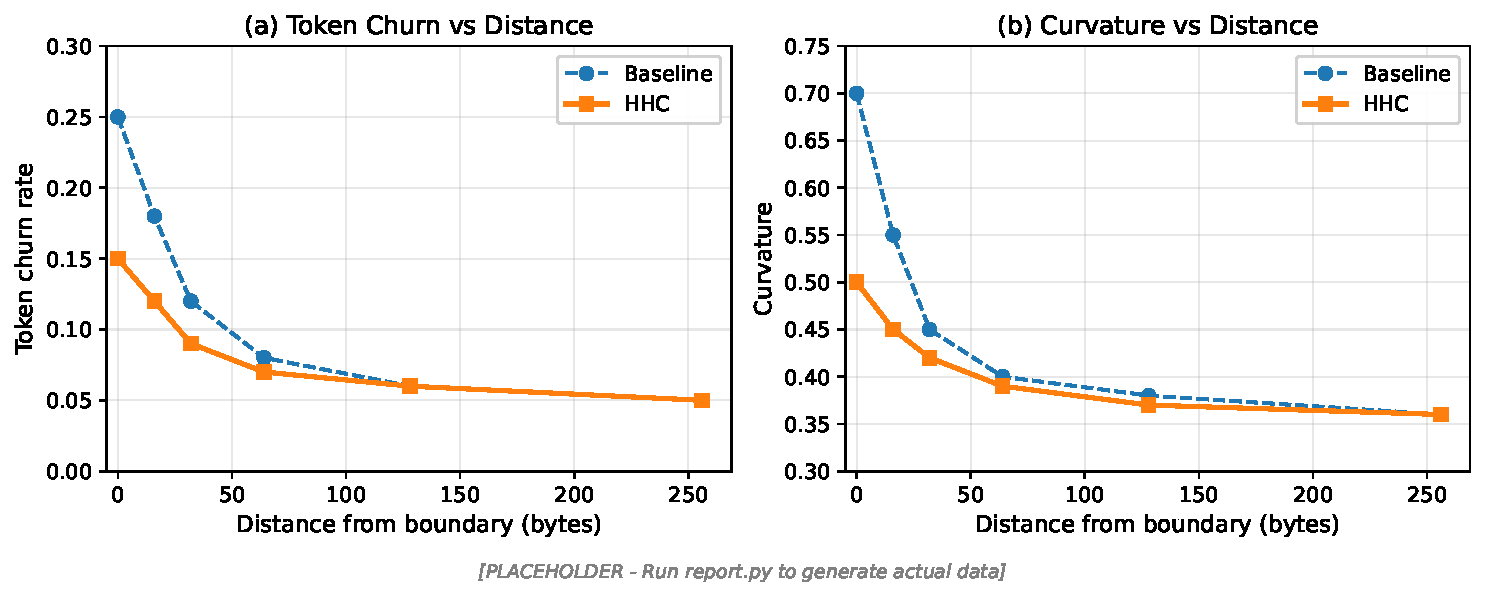
\includegraphics[width=0.9\textwidth]{figures/boundary_analysis.pdf}
\caption{Boundary analysis: churn and curvature vs distance from domain transitions.
Left: Token churn rate decreases with distance from boundary; HHC (solid) shows
reduced churn compared to baseline (dashed) especially at boundaries.
Right: Curvature follows similar pattern; HHC smooths curvature spikes at
domain transitions.}
\label{fig:boundary}
\end{figure}

% Notes for report.py integration:
% - Run: uv run scripts/report.py --compare eval/results/baseline eval/results/hhc
% - This generates results_hhc_tradeoff.tex with populated values
% - Copy values from that file to replace TODO placeholders above
% - Boundary figure data is in boundary_figure_data.json
% - Generate figure with: uv run scripts/generate_boundary_figure.py
